%
% ********************
% *                  *
% *     SECTION 1    *
% *                  *
% ********************
%

\section{Понятие стека. Операции над стеком. Программная реализация стека на основе статического массива}
\subsection{Понятие стека}
Стек~--- абстрактный тип данных, представляющий собой список элементов, организованных по принципу
LIFO (англ. last in -- first out, «последним пришёл -- первым вышел>>). Стеки могут быть построены на основе других, более фундаментальных
структурах данных, например, можно реализовать стек как обертку над массивом с указателем или на основе списка. Проще говоря, стек представляет
собой абстрактный интерфейс доступа к данным, а не конкретную структуру данных.

Организация данных по принципу LIFO означает, что элементы могут добавляться и извлекаться только с вершины стека. При этом при добавлении
элемента, именно он становится новой вершиной стека, а при удалении, вершиной становится предыдущий элемент.

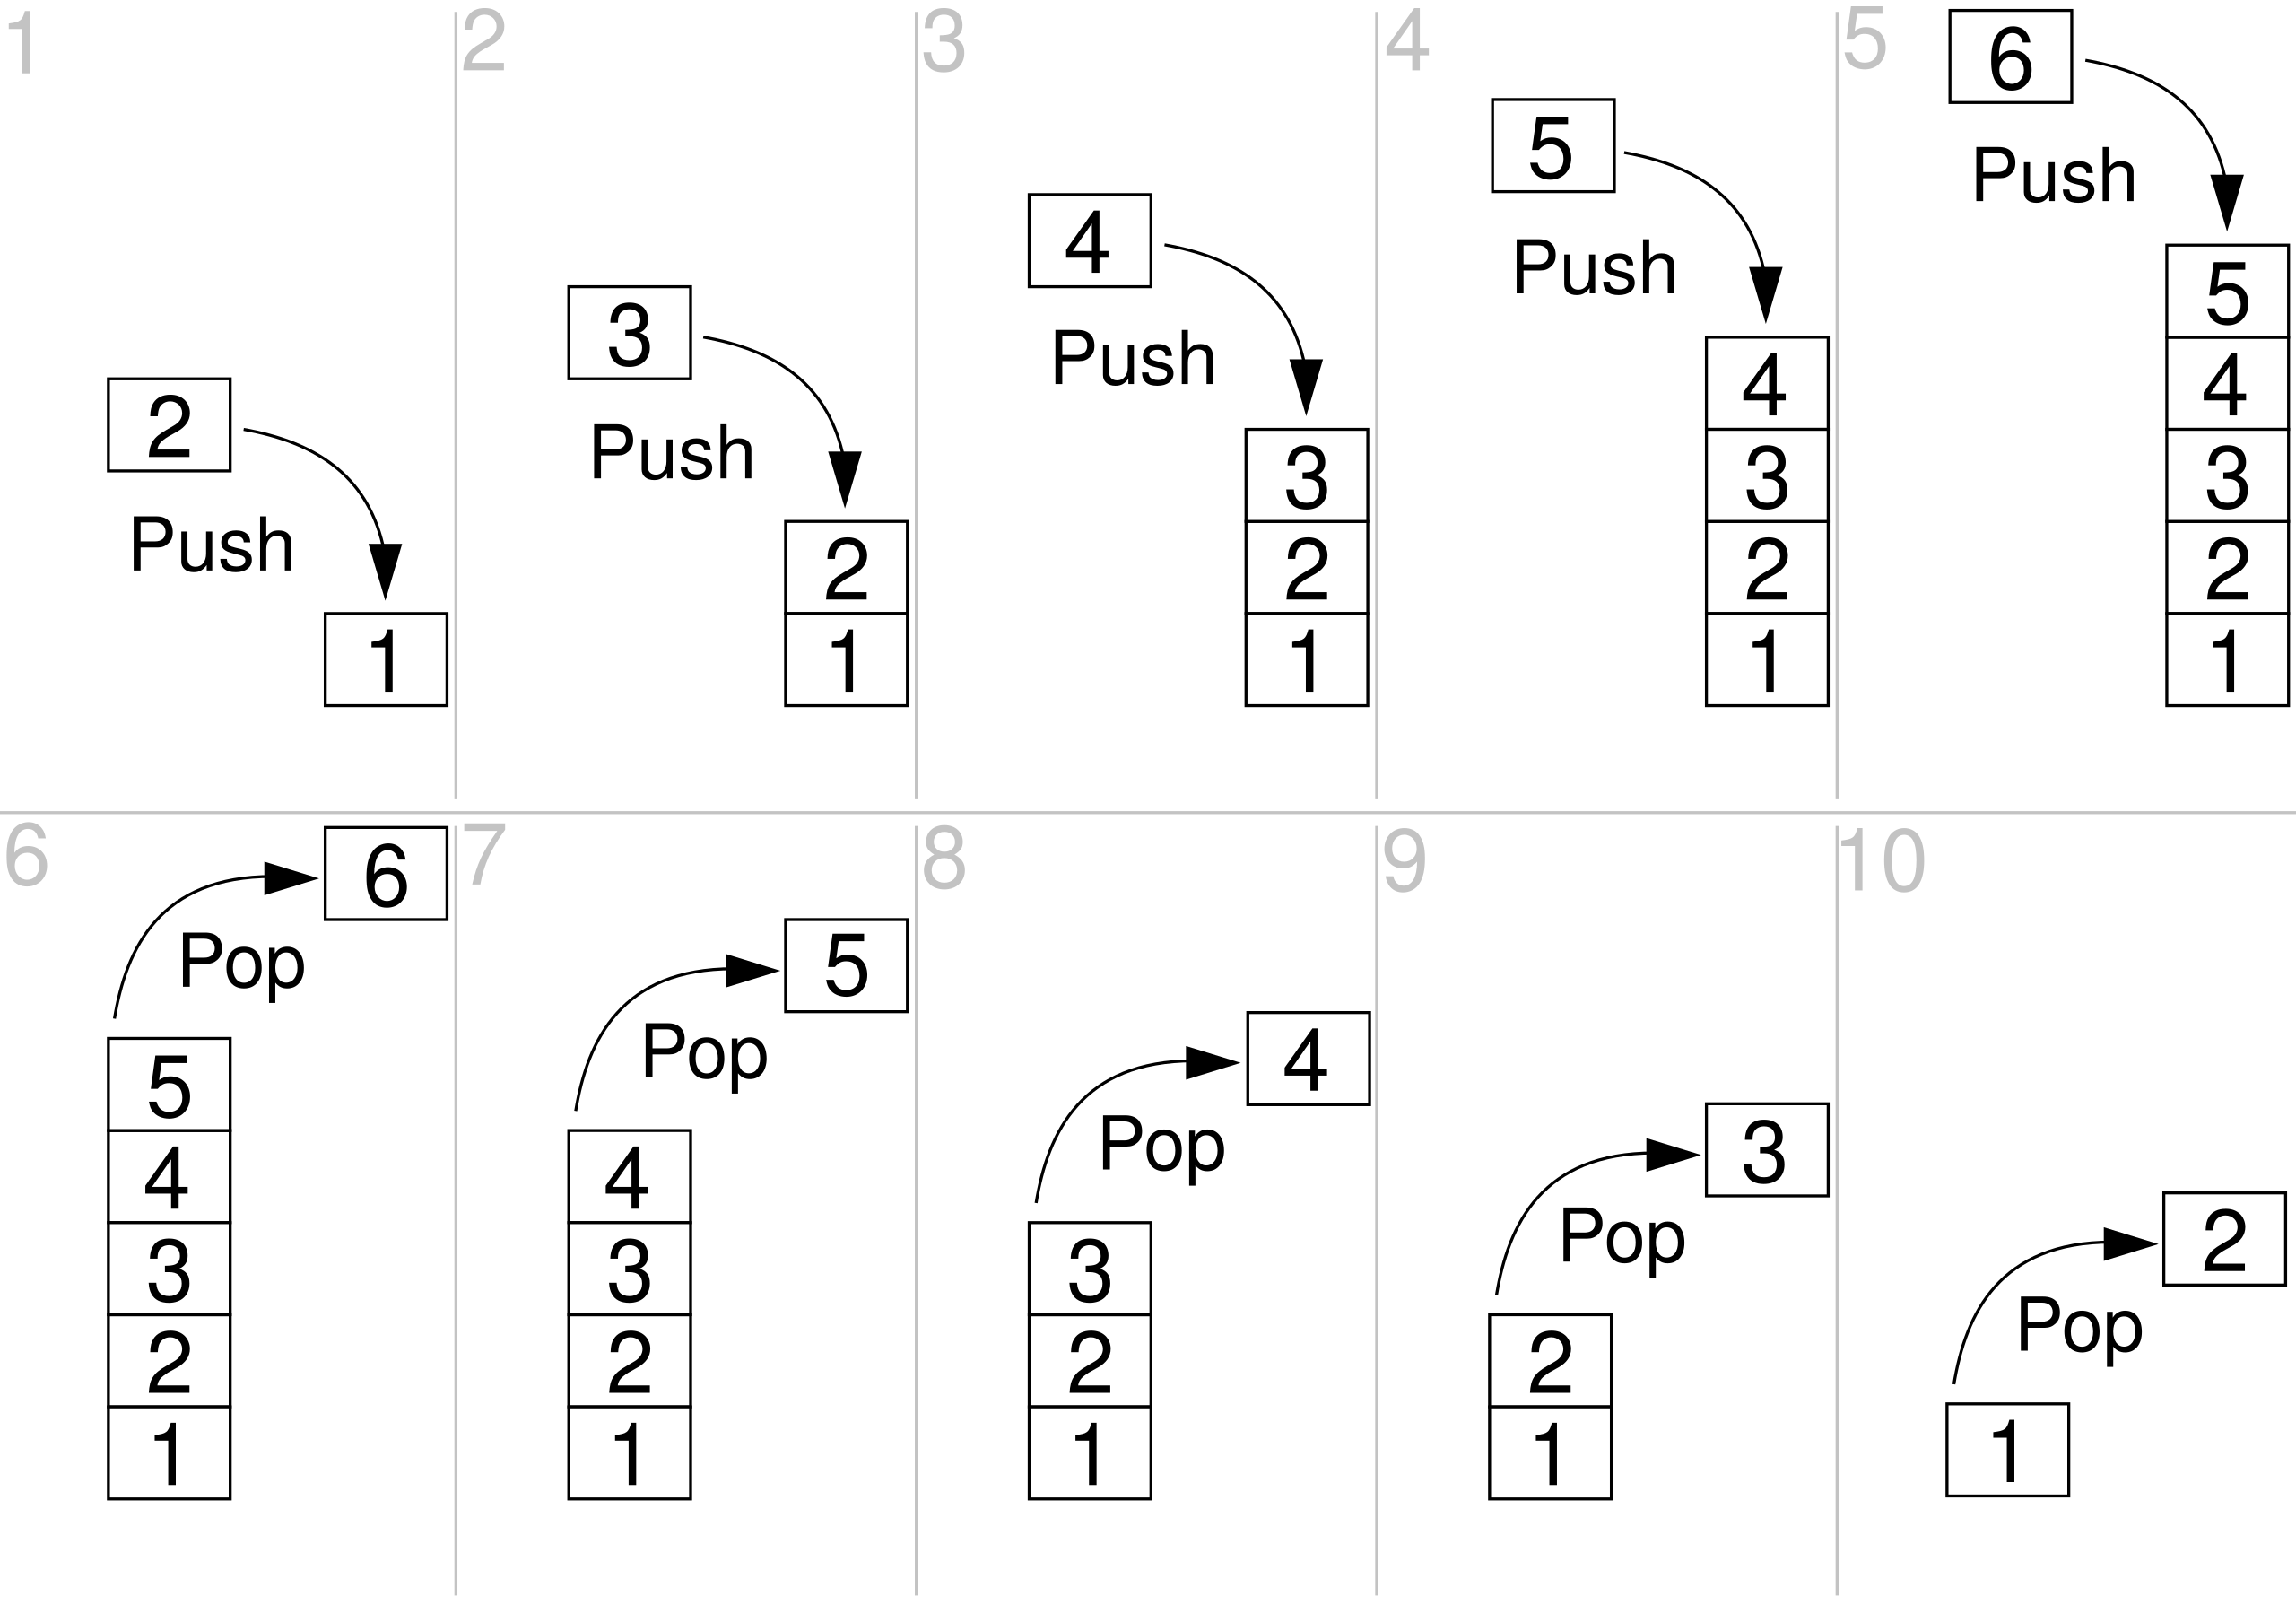
\includegraphics[width=0.9\textwidth]{resources/19-26/stack.png}

В стандартной библиотеке С++ присутствует реализация \cppref[стека]{cpp/container/stack}, объявленная в соответствующем
\cppref[заголовке]{cpp/header/stack}. Стоит отметить, что шаблон \mverb{std::stack<T>} не является
структурой данных сам по себе, а лишь предоставляет интерфейс стека поверх какой-либо другой структуры (по умолчанию, \cppref[\texttt{std::deque<T>}]{cpp/container/deque}).
Помимо этого, в качестве стека можно тривиально использовать динамический массив \cppref[\texttt{std::vector<T>}]{cpp/container/vector} с его
методами \mverb{push_back(T &&)}, \mverb{back()} и \mverb{pop_back()}.
\subsection{Операции над стеком}
Когда речь идет о стеке, подразумевается структура данных со следующими операциями:
\begin{enumerate}
  \item Добавить элемент в верхушку стека (\mverb{push()}).
  \item Удалить элемент из верхушки стека (\mverb{pop()}).
\end{enumerate}

Часто также требуется поддержка операции чтения вершины без ее удаления (\mverb{peek()}, также \mverb{top()}) и
проверки на пустоту (\mverb{empty()}). В эффективной реализации все вышеназванные операции имеют временную сложность
\(O(1)\).

\subsection{Пример реализации стека}
Приведем реализацию стека (С++ 11) на основе статического массива фиксированной длины. Данная реализация будет использовать шаблоны и
\cppref[\texttt{assert(bool)}]{cpp/error/assert} для проверок инвариантов.

\begin{minted}{C++}
template <typename T, size_t N> class Stack {
public:
  Stack() = default;
  ~Stack() = default;

  bool empty() const { return count_ == 0; }
  size_t capacity() const { return N; }
  size_t count() const { return count_; }

  const T &Peek() const {
    assert(count_ > 0 && "Stack is empty.");
    return data_[count_ - 1];
  }
  T &Peek() {
    assert(count_ > 0 && "Stack is empty.");
    return data_[count_ - 1];
  }

  T Pop() {
    assert(count_ > 0 && "Stack is empty.");
    --count_;
    return data_[count_];
  }
  void Push(const T &item) {
    assert(count_ < N && "Stack is full.");
    data_[count_] = item;
    ++count_;
  }
  void Push(T &&item) {
    assert(count_ < N && "Stack is full.");
    data_[count_] = item;
    ++count_;
  }

  T *begin() { return data_; }
  T *end() { return data_ + count_; }
  const T *begin() const { return data_; }
  const T *end() const { return data_ + count_; }

private:
  T data_[N];
  size_t count_{};
};
\end{minted}

%
% ********************
% *                  *
% *     SECTION 2    *
% *                  *
% ********************
%

\section{Понятие очереди. Операции над очередями. Кольцевая очередь. Деки.  Программная реализация очереди на основе статического массива}
Очередь~--- абстрактный тип данных, представляющий собой список данных, организованных по принципу FIFO (англ. first in -- first out, <<первым пришел первым вышел>>).
Очереди могут быть построены на основе других, более фундаментальных структурах данных. Например, очередь может быть внутренне реализована как
список. Об очереди можно судить скорее как об интерфейсе доступа к данным.

Организация по принципу FIFO означает, что элементы могут извлекаться с одного конца (головы), а добавляться~--- с другого (хвоста).

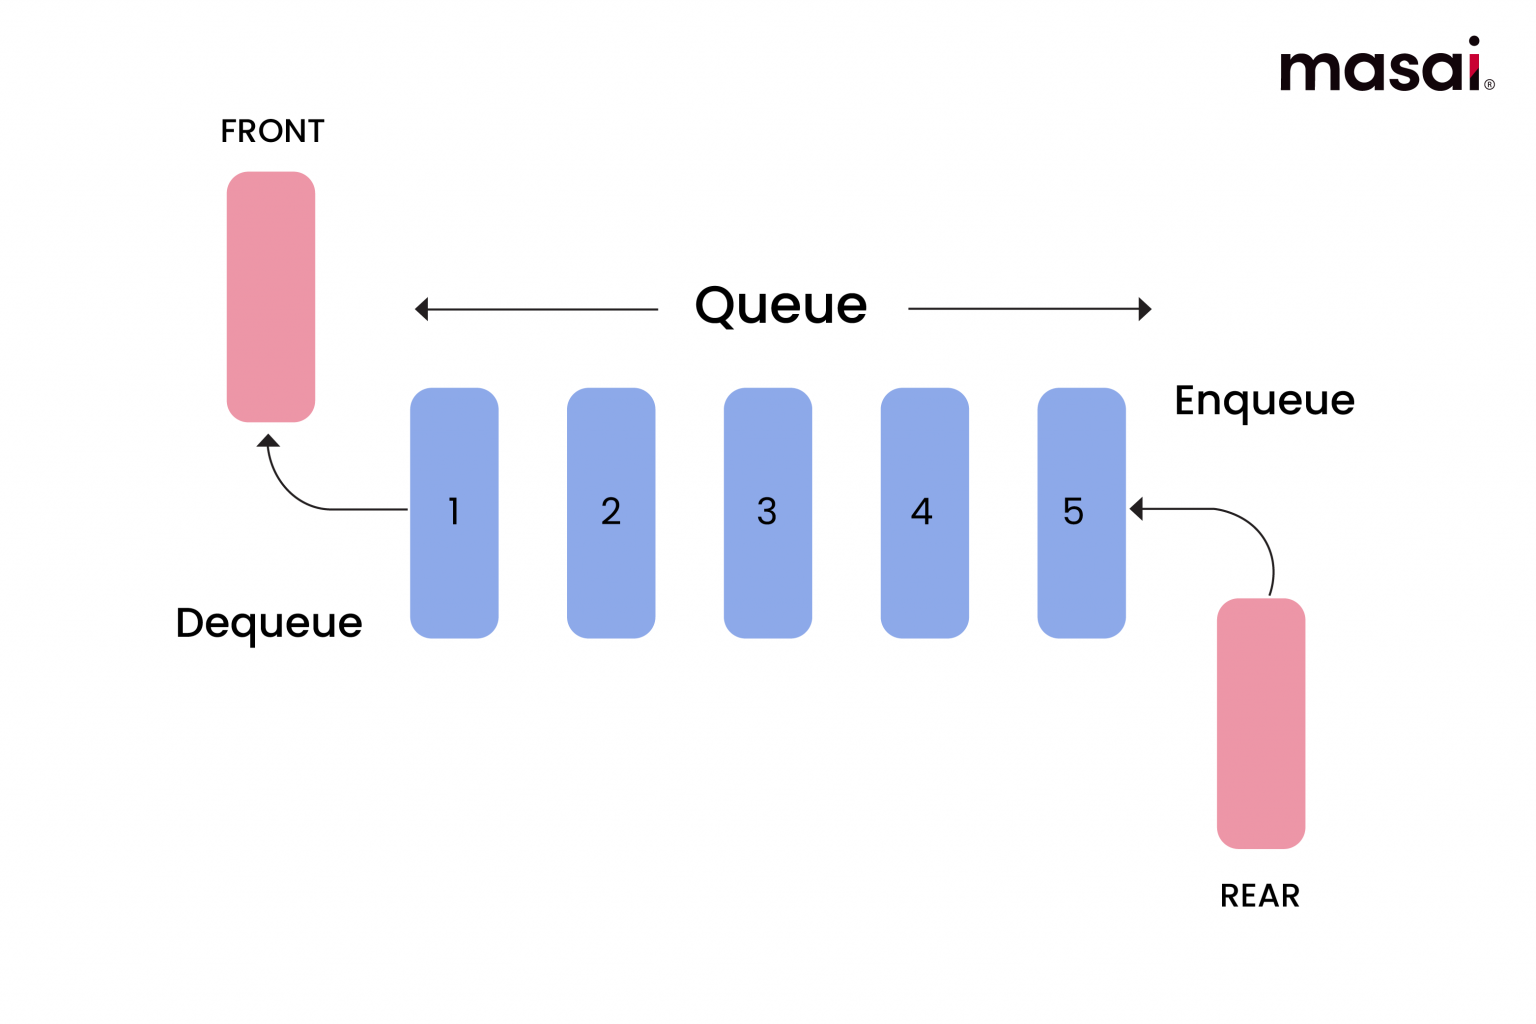
\includegraphics[width=0.9\textwidth]{resources/19-26/queue.png}

В стандартной библиотеке C++ присутствует \cppref[шаблон класса]{cpp/container/queue} \mverb{std::queue<T>}, который является оберткой поверх
какого-либо другого контейнера (по умолчанию, \cppref[\texttt{std::deque<T>}]{cpp/container/deque}).

\subsection{Операции над очередями}
Когда речь идет об очереди, подразумевается структура данных со следующими операциями:
\begin{enumerate}
  \item Добавить элемент в конец (хвост) очереди (\mverb{enqueue()}, в С++ \mverb{push()}).
  \item Удалить элемент из головы очереди (\mverb{dequeue()}, в C++ \mverb{pop()}).
\end{enumerate}
%
Часто также требуется операция чтения головы (\mverb{front()}) и проверки на пустоту (\mverb{empty()}). В эффективной реализации
все указанные операции должны выполнятся за \(O(1)\).

\subsection{Кольцевая очередь}
Кольцевая очередь (кольцевой буфер)~--- очередь (с фиксированным размером), в которой голова и хвост соединены.

\begin{center}
  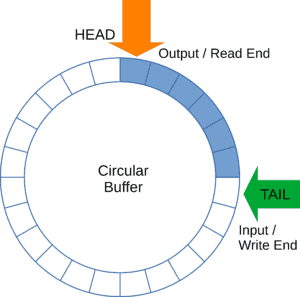
\includegraphics[width=0.3\textwidth]{resources/19-26/ring.png}
\end{center}

Кольцевая очередь может быть эффективно реализована на основе массива с двумя указателями: один для чтения, второй~--- для записи.

Кольцевой буфер находит очень широкое применение в том числе при программировании микроконтроллеров.
Данные структуры часто используют для организации различных очередей сообщений и буферов приёма-передачи различных
коммуникационных интерфейсов. Такая структура также легко предоставляет возможность буферизации потоков данных.

\subsection{Deque}
Дек (англ. deque, double-ended queue)~--- абстрактный тип данных, в котором элементы можно добавлять и удалять как в начало, так и в конец.
От дека требуются следующие операции (работают за \(O(1)\) в эффективной реализации):
\begin{enumerate}
  \item Вставка в начало (\mverb{push_front()}).
  \item Вставка в конец (\mverb{push_back()}).
  \item Удаление из начала (\mverb{pop_front()}).
  \item Удаление с конца (\mverb{pop_back()}).
\end{enumerate}

Помимо этого, существуют варианты деков, поддерживающих также произвольный доступ за \(O(1)\), в частности, такую асимптотическую
сложность гарантирует \cppref[\texttt{std::deque<T>}]{cpp/container/deque}.

\subsection{Реализация очереди}
Приведем реализацию очереди (С++ 11) на основе кольцевого буфера. Реализация использует шаблоны и \cppref[\texttt{assert(bool)}]{cpp/error/assert}
для проверки инвариантов. Также, в данной реализации запрещена перезапись старых данных~--- в этом случае срабатывает \mverb{assert(bool)} \footnote{Можно заметить, что в операциях с очередью над кольцевым буфером используется операция взятия остатка от деления. Это сравнительно
  медленная операция. Если размер очереди (беззнаковое целое) представляет собой степень \(2\), эту операцию можно заменить на побитовое И. Впрочем, современные
  компиляторы делают это автоматически.}.

\begin{minted}{C++}
template <typename T, size_t N> class Queue {
public:
  Queue() = default;
  ~Queue() = default;

  bool empty() const { return count_ == 0; }
  size_t capacity() const { return N; }
  size_t count() const { return count_; }

  T &Peek() {
    assert(count_ > 0 && "Queue is empty.");
    return data_[start_];
  }
  const T &Peek() const {
    assert(count_ > 0 && "Queue is empty.");
    return data_[start_];
  }

  void Enqueue(T &&item) {
    assert(count_ < N && "Queue is full.");
    data_[end_] = item;
    end_ = (end_ + 1) % N;
    ++count_;
  }
  void Enqueue(const T &item) {
    assert(count_ < N && "Queue is full.");
    data_[end_] = item;
    end_ = (end_ + 1) % N;
    ++count_;
  }

  T Dequeue() {
    assert(count_ > 0 && "Queue is empty.");
    T item = data_[start_];
    start_ = (start_ + 1) % N;
    --count_;
    return item;
  }

private:
  T data_[N];
  size_t start_{};
  size_t end_{};
  size_t count_{};
};
\end{minted}


%
% ********************
% *                  *
% *     SECTION 3    *
% *                  *
% ********************
%

\section{Использование очередей при реализации запросов ввода-вывода. Структура данных «список»}
Очередь~--- абстрактный тип данных, представляющий собой список данных, организованных по принципу FIFO (англ. first in -- first out, <<первым пришел первым вышел>>).

Стандартно использование очередей при обработке запросов. Если запросы поступают быстрее, чем обрабатываются, возникает риск потери данных.
Очереди позволяют нивелировать эту проблему~--- все приходящие запросы складываются в очередь и обрабатываются в порядке прихода по мере возможности.

Рассмотрим пример на основе системы ввода-вывода. Вообразим систему, состоящую из клавиатуры, терминала и микроконтроллера на соответствующей
системной плате. Пусть на этом компьютере запущена программа~--- текстовый редактор. Если скорость обработки нажатых клавиш
микроконтроллера достаточно мала, то при быстрой печати он просто не сможет регистрировать некоторые из нажатых клавиш.
Это создает неудобства для пользователя, поскольку не дает ему быстро выполнять его (пользователя) работу по набору
какого-либо документа.

Пусть, однако, контроллер клавиатуры теперь не отправляет коды нажатых клавиш напрямую, а размещает их в очереди,
тогда как микроконтроллер их оттуда извлекает и потом обрабатывает.
Теперь проблема нерегистрируемых нажатий решена~--- в случае просадки производительности микроконтроллера все
нажатые клавиши будут обработаны, просто позднее.

Очереди поддерживают следующие основные операции:
\begin{enumerate}
  \item \mverb{enqueue()} (\mverb{push()})~--- вставка элемента в очередь.
  \item \mverb{dequeue()} (\mverb{pop()})~--- извлечение элемента из очереди.
  \item \mverb{peek()} (\mverb{front()})~--- просматривает голову очереди без извлечения элемента.
  \item \mverb{empty()}~--- проверяет, пуста ли очередь.
\end{enumerate}

Для очередей произвольной длины особенно эффективна реализация на основе связных списков. Приведем такую реализацию:

\begin{minted}{C++}
template <typename T> class ListQueue {
  struct ListQueueNode {
    T item;
    ListQueueNode *n{};
  };

public:
  ListQueue() = default;
  ~ListQueue() {
    while (!Empty()) {
      Dequeue();
    }
  }
  bool Empty() const { return head_ == nullptr; }

  T &Peek() {
    assert(head_ != nullptr && "Queue is empty.");
    return head_->item;
  }
  const T &Peek() const {
    assert(head_ != nullptr && "Queue is empty.");
    return head_->item;
  }

  void Enqueue(const T &item) {
    if (tail_ == nullptr) {
      head_ = tail_ = new ListQueueNode;
      tail_->item = item;
      return;
    }

    ListQueueNode *node = new ListQueueNode;
    node->item = item;
    tail_->n = node;
  }
  void Enqueue(T &&item) {
    if (tail_ == nullptr) {
      head_ = tail_ = new ListQueueNode;
      tail_->item = item;
      return;
    }

    ListQueueNode *node = new ListQueueNode;
    node->item = item;
    tail_->n = node;
    tail_ = node;
  }
  T Dequeue() {
    assert(head_ != nullptr && "Queue is empty.");
    ListQueueNode *node = head_;

    head_ = head_->n;

    T item = node->item;
    delete node;
    return item;
  }

private:
  ListQueueNode *head_{};
  ListQueueNode *tail_{};
};
\end{minted}

Отметим, что названную очередь можно тривиально реализовать как обертку над контейнерами \cppref[\texttt{std::list<T>}]{cpp/container/list} (двусвязный список),
\cppref[\texttt{std::forward\_list<T>}]{cpp/container/forward_list} (односвязный список) или \cppref[\texttt{std::deque<T>}]{cpp/container/deque}.

В многозадачной операционной системе или сервере приложений очередь запросов I/O может помочь:
\begin{itemize}
  \item Сгладить пики нагрузки~--- запросы поступают в очередь и обрабатываются по мере возможности, что позволяет системе справляться с временными пиками нагрузки.
  \item Обеспечить справедливость~--- запросы обрабатываются в порядке поступления, что обеспечивает равные шансы для всех задач.
  \item Управлять приоритетами~--- очереди с приоритетами могут быть использованы для обработки более важных запросов раньше менее важных.
\end{itemize}

%
% ********************
% *                  *
% *     SECTION 4    *
% *                  *
% ********************
%

\section{Программная реализация очереди на основе статического массива}
Очередь~--- абстрактный тип данных, представляющий собой список данных, организованных по принципу FIFO (англ. first in -- first out,
<<первым пришел первым вышел>>).

Одним из простейших способов реализации очереди фиксированной длины с оптимальной асимптотической сложностью основных операций (\(O(1)\) для вставки в конец, \mverb{enqueue}, и
извлечения из начала, \mverb{dequeue}) основана на использовании кольцевого буфера. В такой реализации помимо самого статического массива
хранятся еще два индекса~--- указатели на начало и конец очереди.

\begin{center}
  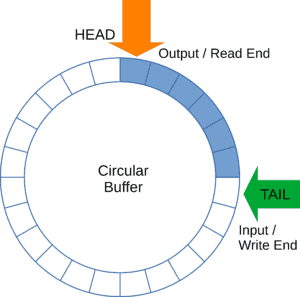
\includegraphics[width=0.3\textwidth]{resources/19-26/ring.png}
\end{center}

Самих двух указателей недостаточно, однако, чтобы отличить пустую очередь от полной. Есть два подхода решения этой проблемы:
\begin{enumerate}
  \item Допустить хранение в очереди не \(N\) элементов, а \(N - 1\), где \(N\)~--- длина массива. Тогда
        очередь заполнена, когда, например, хвост на один индекс меньше головы.
  \item Можно хранить отдельным полем количество элементов в очереди. Тогда очередь пуста, если \mverb{count_ == 0}, и полна, когда
        \mverb{count_ == N}.
\end{enumerate}

Приведем реализацию очереди (С++ 11) на основе статического массива с отдельным счетчиком числа элементов. В данной реализации инварианты проверяются при
помощи \cppref[\texttt{assrt(bool)}]{cpp/error/assert}. Также приведенная очередь является шаблоном по типу элементов и своему размеру
\footnote{Можно заметить, что в операциях с очередью над кольцевым буфером используется операция взятия остатка от деления. Это сравнительно
  медленная операция. Если размер очереди (беззнаковое целое) представляет собой степень \(2\), эту операцию можно заменить на побитовое И. Впрочем, современные
  компиляторы делают это автоматически.}.

\begin{minted}{C++}
template <typename T, size_t N> class Queue {
public:
  Queue() = default;
  ~Queue() = default;

  bool empty() const { return count_ == 0; }
  size_t capacity() const { return N; }
  size_t count() const { return count_; }

  T &Peek() {
    assert(count_ > 0 && "Queue is empty.");
    return data_[start_];
  }
  const T &Peek() const {
    assert(count_ > 0 && "Queue is empty.");
    return data_[start_];
  }

  void Enqueue(T &&item) {
    assert(count_ < N && "Queue is full.");
    data_[end_] = item;
    end_ = (end_ + 1) % N;
    ++count_;
  }
  void Enqueue(const T &item) {
    assert(count_ < N && "Queue is full.");
    data_[end_] = item;
    end_ = (end_ + 1) % N;
    ++count_;
  }

  T Dequeue() {
    assert(count_ > 0 && "Queue is empty.");
    T item = data_[start_];
    start_ = (start_ + 1) % N;
    --count_;
    return item;
  }

private:
  T data_[N];
  size_t start_{};
  size_t end_{};
  size_t count_{};
};
\end{minted}

%
% ********************
% *                  *
% *     SECTION 5    *
% *                  *
% ********************
%

\section{Многократный поиск на основе использования статистических данных\footnote{
    Авторы солидарны с предыдущем потоком ИиТП по поводу глупости этого вопроса, и за не имением лучших
    идей продублируют представленную ранее
    \href{https://docs.google.com/document/d/1IDx1FsePF0Gved69eeGE0gimE9MP1xxI_EY23wfWqO0/edit?tab=t.0}{информацию}.}}

Для улучшения эффективности многократного поиска подстрок в тексте может использоваться
\textit{многократный поиск на основе статистических данных}. В этом случае большим подспорьем может стать информация о частоте
вхождений в текст символов из алфавита. Для заданного образца определяется наименее используемый в строке символ и далее алгоритм
основан на перемещении по образцу с помощью перехода на следующий <<редкий символ>>. При этом такой поиск часто сочетает в себе
элементы традиционных алгоритмов поиска подстроки в строке. Приведем краткие сведения о них.

\subsection{Прямой поиск}
Наивное сопоставление текста с шаблоном. Крайне низкая эффективность (временная сложность \(O(n\cdot m)\), \(n\) и \(m\)~---
длины строки и подстроки соответственно). Приведем псевдокод алгоритма (\textit{needle}~--- шаблон, \textit{haystack}~--- строка).

\begin{algorithmic}
  \Function{$na\ddot\imath ve\_search$}{$needle, haystack$}
  \For{$i \gets 0; haystack\left[i\right] \ne 0; i \gets i + 1 $}
  \For{$j \gets 0; ; j \gets j + 1$}
  \If{$needle\left[j\right] \ne 0$}
  \Return $i$
  \EndIf
  \If{$haystack\left[i + j\right] \ne needle\left[j\right]$}
  \State \textbf{break}
  \EndIf
  \EndFor
  \EndFor
  \State
  \Return $unsuccessful$
  \EndFunction
\end{algorithmic}

\subsection{Алгоритм Кнута-Мориса-Пратта}
Алгоритм КМП~--- эффективный алгоритм поиска подстроки в строке, работающий за линейное время (\(O(n + m)\), \(n\)~--- длина шаблона, \(m\)~--- строки).
Он использует предварительную обработку искомой строки для создания таблицы <<префиксов>>,
которая указывает, куда следует переместить индекс поиска в случае несоответствия символов.

Псевдокод алгоритма:

\begin{algorithmic}
  \Function{$kmp\_search$}{$needle, haystack$}
  \State $j \gets 0$
  \State $k \gets 0$
  \State $T \gets kmp\_table(needle)$
  \While{$j < \text{length}(haystack)$}
  \If{$needle\left[k\right] = haystack\left[j\right]$}
  \State $j \gets j + 1$
  \State $k \gets k + 1$
  \If{$k = \text{length}(needle)$}
  \Return $j - k$
  \Else
  \State $k \gets T\left[k\right]$
  \If{$k < 0$}
  \State $j \gets j + 1$
  \State $k \gets k + 1$
  \EndIf
  \EndIf
  \EndIf
  \EndWhile
  \State
  \Return $unsuccessful$
  \EndFunction\\

  \Function{$kmp\_table$}{$needle$}
  \State $T \gets \left[\right]$
  \State $pos \gets 1$
  \State $cnd \gets 0$
  \While{$pos < \text{length}(needle)$}
  \If{$needle\left[pos\right] = needle\left[cnd\right]$}
  \State $T\left[pos\right] \gets T\left[cnd\right]$
  \Else
  \State $T\left[pos\right] \gets cnd$
  \While{$cnd \ge 0~\textbf{and}~needle\left[pos\right] \ne needle\left[cnd\right]$}
  \State $cnd \gets T\left[cnd\right]$
  \EndWhile
  \EndIf
  \State $pos \gets pos + 1$
  \State $cnd \gets cnd + 1$
  \EndWhile
  \State
  \Return $T$
  \EndFunction
\end{algorithmic}

Дополнительно можно изучить по ссылкам: \href{https://en.wikipedia.org/wiki/Knuth\%E2\%80\%93Morris\%E2\%80\%93Pratt_algorithm}{Wikipedia},
\href{https://neerc.ifmo.ru/wiki/index.php?title=\%D0\%90\%D0\%BB\%D0\%B3\%D0\%BE\%D1\%80\%D0\%B8\%D1\%82\%D0\%BC\_\%D0\%9A\%D0\%BD\%D1\%83\%D1\%82\%D0\%B0-\%D0\%9C\%D0\%BE\%D1\%80\%D1\%80\%D0\%B8\%D1\%81\%D0\%B0-\%D0\%9F\%D1\%80\%D0\%B0\%D1\%82\%D1\%82\%D0\%B0}{Итмо}.

\subsection{Алгоритм Бойера-Мура-Хорспула}
Этот эффективный алгоритм поиска подстроки в строке на практике оказывается быстрее других. В среднем (почти всегда) имеет линейное
время работы (\(O(n + m)\), \(n\)~--- длина шаблона, \(m\)~--- строки); однако на определенных наборах данных
может деградировать до \(O(n\cdot m)\). В отличие от большинства других алгоритмов, алгоритм Бойера-Мура-Хорспула сравнивает
символы с конца, а не с начала, как большинство других алгоритмов.

Алгоритм предварительно обрабатывает данные, строя таблицы для эвристик. После чего на стадии поиска эти эвристики используются
для ускорения нахождения следующего возможного совпадения.

Дополнительная информация: \href{https://neerc.ifmo.ru/wiki/index.php?title=Алгоритм_Бойера-Мура}{Итмо},
\href{https://ru.wikipedia.org/wiki/Алгоритм_Бойера_—_Мура_—_Хорспула}{Википедия}.

%
% ********************
% *                  *
% *     SECTION 6    *
% *                  *
% ********************
%

\section{Нечеткий поиск – поиск <<подобной>> подстроки. Бинарный поиск}

\subsection{нечеткий поиск}
Задача нечеткого поиска (fuzzy string search)~--- найти в тексте или словаре (\textit{haystack}) все подстроки, совпадающие
(начинающиеся) с данной (\textit{needle}) с учетом не более \(k\) ошибок.
Эти алгоритмы являются основными в системах коррекции наборных ошибок
(например \href{https://en.wikipedia.org/wiki/Code_completion}{автодополнение кода} в IDE или подсказки в поисковой строке браузера).
В зависимости от преследуемых целей, существуют и используются различные алгоритмы решения данной задачи в различных постановках.

\subsubsection{Метрики Левенштейна и Хэмминга}
Расстояние Левенштейна~--- минимальное количество односимвольных операций (а именно вставки, удаления, замены),
необходимых для превращения одной последовательности символов в другую.
% cSpell: disable-next-line
Например, расстояние Левенштейна слов \(L(Hello, Hilo) = 2\) (замена `\(e\)' \(\gets\) `\(i\)', вставка `\(l\)').

Расстояние Хэмминга~--- число позиций, в которых соответствующие символы двух слов одинаковой длины различны. Например,
% cSpell: disable-next-line
\(H(Hello, Hillo) = 1\) (замена `\(e\)' \(\gets\) `\(i\)').

Расстояния Хэмминга и Левенштейна, во-первых, являются метриками в математическом смысле слова, во-вторых, позволяют строго
формализовать задачу нечеткого поиска.

Расстояние Левенштейна можно вычислить на основе рекуррентной формулы \[L(a,b) = \begin{cases}
    |a|                                  & \text{если}~|b| = 0,                         \\
    |b|                                  & \text{если}~|a| = 0,                         \\
    L(\text{tail}(a), \text{tail}(b))    & \text{если}~\text{head}(a) = \text{head}(b), \\
    1 + \min \begin{cases}
               L(\text{tail}(a), b)              \\
               L(a, \text{tail}(b))              \\
               L(\text{tail}(a), \text{tail}(b)) \\
             \end{cases} & \text{иначе}                                          \\
  \end{cases}
\]

где \(\text{tail}(\overline{x_1x_2x_3\dots}) = \overline{x_2x_3\dots}\), а \(\text{head}(\overline{x_1x_2x_3\dots}) = x_1\).
Используя также мемоизацию на матрице, можно вычислить расстояние Левенштейна между любыми двумя строками длины \(n\) и \(m\) за
\(O(n\cdot m)\)~--- алгоритм \href{https://neerc.ifmo.ru/wiki/index.php?title=%D0%97%D0%B0%D0%B4%D0%B0%D1%87%D0%B0_%D0%BE_%D1%80%D0%B5%D0%B4%D0%B0%D0%BA%D1%86%D0%B8%D0%BE%D0%BD%D0%BD%D0%BE%D0%BC_%D1%80%D0%B0%D1%81%D1%81%D1%82%D0%BE%D1%8F%D0%BD%D0%B8%D0%B8,_%D0%B0%D0%BB%D0%B3%D0%BE%D1%80%D0%B8%D1%82%D0%BC_%D0%92%D0%B0%D0%B3%D0%BD%D0%B5%D1%80%D0%B0-%D0%A4%D0%B8%D1%88%D0%B5%D1%80%D0%B0}{Вагнера-Фишера}.

\subsubsection{Алгоритм bitap}
Алгоритм \href{https://en.wikipedia.org/wiki/Bitap_algorithm}{bitap} позволяет эффективно с точки зрения реального времени работы процессора вычислять расстояние Хэмминга и
(с модификациями) Левенштейна. При асимптотике \(O(k\cdot n)\), он работает ощутимо быстрее наивного вычисления метрики
Левенштейна для сравнения двух строк, поскольку сравнивает по 32/64 символа за раз. Фактически, это эффективное
распараллеливание наивного линейного алгоритма.

\subsubsection{Алгоритм расширенной выборки}
\begin{center}
  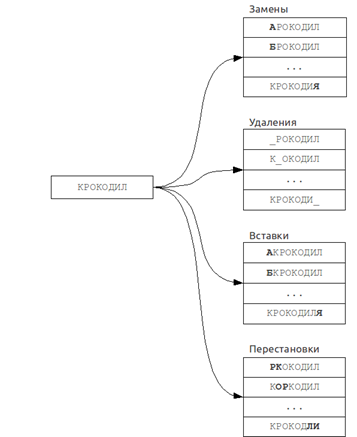
\includegraphics[width=0.3\textwidth]{resources/19-26/inflate.png}
\end{center}
Сводит задачу нечеткого поиска к задаче точного поиска последовательным перебором всех ошибочных трансформаций входной строки.
Неэффективен на больших алфавитах и при больших \(k\), даже при бинарном поиске по словарю временная сложность
\(O((m\cdot |\Sigma|)^k\cdot m\cdot \log{n})\), где \(|\Sigma|\)~--- размер алфавита.

\subsubsection{Метод \(N\)-грамм}
\begin{center}
  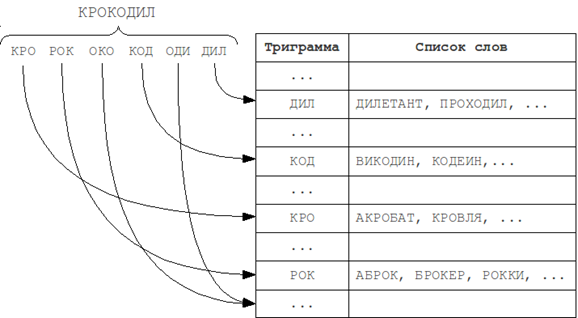
\includegraphics[width=0.3\textwidth]{resources/19-26/n-gramms.png}
\end{center}

Основан на разбиении всех слов в словаре и исходного на \(N\)-граммы~--- последовательности длины \(N\) (обычно \(N = 3\)).
\(N\)-граммы используются для группировки слов в корзины, по которым в дальнейшем и производится поиск.

\subsubsection{\href{https://cs.msu.ru/sites/cmc/files/docs/boycov.pdf}{Хеширование по сигнатуре}, \href{https://en.wikipedia.org/wiki/Locality-sensitive_hashing\#Bit_sampling_for_Hamming_distance}{Locality-sensitive hashing}}

\begin{center}
  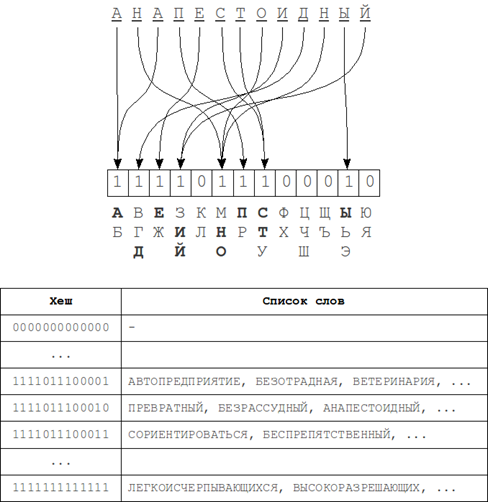
\includegraphics[width=0.3\textwidth]{resources/19-26/hash.png}
\end{center}
Предполагают сопоставление каждому слову специального хеша так, что схожие слова имеют схожие хеш-функции. Тогда поиск следует вести с
теми словами в словаре, у которых близкий или одинаковый хеш с исходной строкой.

\subsection{Бинарный поиск}
Бинарный поиск (также логарифмический поиск)~--- эффективный алгоритм поиска в упорядоченных данных с произвольным доступом
(обычно это отсортированный массив). Выполняется путем деления диапазона поиска пополам.

Приведем псевдокод и словесное описание данного алгоритма:
\begin{algorithmic}
  \Function{$binary\_search$}{$A, n, T$}
  \State $L \gets 0$
  \State $R \gets n - 1$
  \While{$L \le R$}
  \State $m \gets L + \lfloor\frac{R - L}{2}\rfloor$
  \If{$A\left[n\right] < T$}
  \State $L \gets m + 1$
  \ElsIf{$A\left[n\right] > T$}
  \State $R \gets m - 1$
  \Else
  \State \Return $m$
  \EndIf
  \EndWhile
  \State \Return $unsuccessful$
  \EndFunction
\end{algorithmic}

\bigbreak

Первоначально интервал поиска~--- вся коллекция.
Затем на каждой итерации:
\begin{itemize}
  \item проверка концов интервала: если значение/ключ совпали, то
        искомый элемент найден;
  \item проверка длины интервала: если начало совпадает с концом, то
        поиск завершен неуспешно;
  \item вычисление середины интервала (по индексам!)~--- это будет
        медианное значение текущего интервала;
  \item проверка точного попадания в медианное значение;
  \item в зависимости от того, больше или меньше медианы искомое
        значение, повтор поиска для правого или левого подинтервала.
\end{itemize}

Таким образом, на каждой итерации объем данных, требующих анализа, сокращается вдвое~---
логарифмическая (очень оптимистичная!) зависимость трудоемкости от объема набора.

%
% ********************
% *                  *
% *     SECTION 7    *
% *                  *
% ********************
%

\section{Рекурсия: общий вид, свойства, проблемы. Стек вызова функций}
Рекурсия~--- метод решения вычислительной задачи, при котором решение зависит от решения меньших подзадач того же рода. Такие задачи решаются
при помощи функций (методов), вызывающих самих себя для меньших объемов данных.

Можно доказать, что рекурсия по вычислительной способности эквивалентна программам с циклами, что делает
рекурсию мощным инструментом решения алгоритмических задач\footnote{Существуют языки программирования (например, Haskell или Clojure),
  в которых рекурсия является единственным способом повторно вызывать код. При этом такие языки по своем вычислительной
  способности эквивалентны более традиционным языкам.}.

Чтобы функция была рекурсивной, необходимо и достаточно наличие в этой функции вызова самой себя при каких-либо путях выполнения кода. При этом
не обязательно, чтобы вызов функции самой себя был указан напрямую в теле этой функции (\textit{прямая рекурсия}), рекурсивный вызов может
выполнятся и в какой-либо другой функции, вызываемой данной (\textit{косвенная рекурсия}).

У рекурсии, как метода решения алгоритмических задача, есть определенные достоинства и недостатки:
\begin{itemize}
  \item Простота~--- рекурсивные решения часто проще и элегантнее итеративных.
  \item Мощность~--- рекурсивные решения эквивалентны итеративным, причем некоторые задачи гораздо проще решить
        именно рекурсивным способом.
  \item Накладные расходы~--- вызов функций имеет определенные временные затраты, заметные в случае сравнительно
        простых для вычисления функций. Тогда временные затраты на вызовы будут занимать существенное по сравнению с
        полезными вычислениями время.
  \item Проблема переполнения стека~--- вызов функций, требующий дополнительную память сопряжен риском исчерпания машинного стека
        вызова и аварийного завершения программы при достаточно большом объеме входных данных и высокой глубине рекурсии.
\end{itemize}

\subsection{Классификация рекурсии}
Рекурсия может быть классифицирована по различным признакам:
\begin{enumerate}
  \item По типу вызова
        \begin{itemize}
          \item Прямая рекурсия~--- функция взывает саму себя непосредственно.
          \item Косвенная рекурсия~--- функция вызывает функцию, которая вызывает исходную.
        \end{itemize}
  \item По структуре вызова
        \begin{itemize}
          \item Хвостовая рекурсия~--- если рекурсивный вызов является последней операции перед возвратом из функции.
          \item Нехвостовая рекурсия~--- в противном случае.
        \end{itemize}
  \item По направлению вызова
        \begin{itemize}
          \item Нисходящая рекурсия~--- функция решает задачу рекурсивно, вызываясь для все меньших и меньших входных данных. После
                достижения базового случая, рекурсивные вызовы возвращают, объединяя результаты для получения решения исходной проблемы.
          \item Восходящая рекурсия~--- рекурсивная функция постепенно создает решение, начиная с простейшей задачи и
                передавая промежуточные результаты дальнейшим рекурсивным вызовам. С каждым вызовом вычисляется решение для все больших
                входных данных, пока, наконец, не будет получено решение исходной задачи. Восходящая рекурсия обычно также хвостовая.
        \end{itemize}
  \item По степени ветвления
        \begin{itemize}
          \item Линейная~--- рекурсивные вызовы на любом рекурсивном срезе, инициируют не более одного последующего рекурсивного вызова.
          \item Нелинейная рекурсия~--- в противном случае.
        \end{itemize}
\end{enumerate}

Приведем несколько примеров:
\begin{minted}{C++}
// Рекурсивное вычисление факториала числа
// Пример прямой нехвостовой нисходящей линейной рекурсии
int32_t Factorial(int32_t n) {
  return n <= 1 ? 1 : n * factorial(n - 1);
}

// Еще один факториал, оптимизированная версия
// Пример прямой хвостовой восходящей линейной рекурсии
int32_t FactorialRec(int32_t n, int32_t acc) {
  return n <= 1 ? 1 : FactorialRec(n - 1, n * acc);
}
int32_t BetterFactorial(int32_t n) {
  return FactorialRec(n, 1);
}

// Вычисление суммы всех элементов в двоичном дереве
// Пример прямой нехвостовой нисходящей нелинейной рекурсии
int32_t Sum(Node *node) {
  if (node == nullptr) {
    return 0;
  }

  int32_t left = Sum(node->left);
  int32_t right = Sum(node->right);

  return left + node->value + right;
}
\end{minted}

\subsection{Стек вызова функций}
Стек вызова (от англ. call stack)~--- LIFO-стек, хранящий информацию для возврата
управления из подпрограмм (процедур, функций) в программу
(или подпрограмму, при вложенных или рекурсивных вызовах).

Организация стека вызовов регламентируется двоичным интерфейсом платформы (в частности, операционной системой,
применяемым соглашением о вызовах). Также стек вызовов зачастую имеет аппаратную поддержку\footnote{на x86-64 есть инструкции \texttt{push} и \texttt{pop}, которые
  манипулируют машинным стеком. Они предполагают, что на вершину стека указывает регистр \texttt{esp}/\texttt{rsp}. Так же стек используют
  инструкции \texttt{call} и \texttt{ret}; обо всем этом можно почитать в \href{https://www.cs.cmu.edu/~410/doc/intel-isr.pdf}{мануале Intel}.
}.

Когда производится вызов процедуры или функции, адрес следующей за ней инструкции (\textit{адрес возврата}) сохраняется в стеке. Также в
стеке сохраняются все (или только часть, зависит от \href{https://en.wikipedia.org/wiki/Calling_convention}{соглашения о вызовах})
аргументы, возможно, локальные переменные вызывающей (\textit{caller}) подпрограммы. После чего управление передается в вызываемую
подпрограмму (\textit{callee}). По завершении вызываемой подпрограммы, из стека извлекается адрес возврата и все данные \textit{callee},
после чего выполнение \textit{caller} продолжается.

Область памяти стека, ассоциированная с конкретным вызовом конкретной подпрограммы часто называется стековым кадром, или кадром стека.
Кадр стека хранит адрес возврата, локальные переменные, сохраненные регистры, аргументы подпрограммы.

С помощью стека вызовов обеспечивается возможность написания гибкого кода: поддержка рекурсии, подпрограмм в подпрограммах, вызов функций
с многими аргументами.

%
% ********************
% *                  *
% *     SECTION 8    *
% *                  *
% ********************
%

\section{Сортировки – общая классификация. Сортировки с помощью включения, выделения, обменов}
Сортировка~--- процесс упорядочивания данных в соответствии с заданным критерием.

Сортировка является фундаментальной операцией при работе с данными, поскольку позволяет работать с ними более
эффективно. В частности, если данные отсортированы, становятся возможным использовать эффективные алгоритмы поиска.

\subsection{Радикальные подходы}
Сортировку можно выполнить аппаратно если число элементов данных невелико~--- строится схема-сортировщик из ячеек памяти
со связями <<каждый с каждым>>, после чего одного прохода достаточно для упорядочивания данных. Очень
неэффективно на больших объемах данных, но очень удобно (и быстро), на малых (например, несколько чисел).

Другая крайность представляет собой перегон элементов в естественно упорядоченную структуру данных~--- двоичное дерево поиска.
После производится обход дерева с извлечением элементов в отсортированном порядке.
Асимптотическая сложность таких алгоритмов даже может быть очень неплохой\footnote{
  Одна из таких сортировок~--- \href{https://en.wikipedia.org/wiki/Splaysort}{splaysort}, использует особое
  сбалансированное дерево поиска~--- \href{https://en.wikipedia.org/wiki/Splay_tree}{splay-дерево}. Такое дерево постоянно перестраивает
  само себя, адаптируясь ко входным данным, работая фактически как кеш. Можно показать, что splaysort работает в среднем не хуже
  \(O(n\log{n})\), а если данные уже частично упорядоченны~--- то даже еще лучше.
}, но основным и серьезным недостатком является
необходимость в \(O(n)\) дополнительной памяти на хранение дерева, при том что данные в дереве дублируют исходные.

Теперь прейдем к классическим алгоритмам сортировки и их классификации.
\subsection{Классификация алгоритмов сортировки}
Алгоритмы сортировки делятся на группы по различным критериям:
\begin{enumerate}
  \item По методике сортировки \begin{itemize}
          \item Внешние~--- сортируют данные на внешних носителях (пример: сортировка слиянием на внешних устройствах).
          \item Внутренние~--- сортирую данные в оперативной памяти.
        \end{itemize}
  \item По способу реализации
        \begin{itemize}
          \item Сортировка обменом~--- выявление пар элементов, нарушающих порядок сортировки, и обмен местами.
                В обычных последовательных реализациях подход неэффективен, но могут быть хорошо приспособлены для
                параллельной реализации.\\
                \textbf{Примеры}: <<пузырьковая>> сортировка, \href{https://en.wikipedia.org/wiki/Bitonic_sorter}{битонная} (параллельная) сортировка.
          \item Сортировка выбором~--- последовательный поиск и отделение от остальных элементов в порядке сортировки.\\
                \textbf{Примеры}: \href{https://en.wikipedia.org/wiki/Selection_sort}{сортировка выбором}.
          \item Сортировка вставками~--- последовательный просмотр элементов (из числа еще неупорядоченных) и вставка их
                на соответствующее им место среды уже упорядоченных.\\
                \textbf{Примеры}: сортировка вставками, \href{https://en.wikipedia.org/wiki/Shellsort}{сортировка Шелла}.
        \end{itemize}
  \item По стабильности \begin{itemize}
          \item Стабильные~--- гарантируют относительный порядок равных элементов (пример: сортировка вставками).
          \item Нестабильные~--- в противном случае (пример: быстрая сортировка).
        \end{itemize}
  \item По использованию дополнительной памяти \begin{itemize}
          \item In-place~--- дополнительная память не требуется (пример: пирамидальная сортировка).
          \item Out-of-place~--- в противном случае (пример: сортировка слиянием).
        \end{itemize}
  \item По адаптивности \begin{itemize}
          \item Адаптивные~--- работают быстрее с частично отсортированными данными (пример: сортировка вставками, \href{https://en.wikipedia.org/wiki/Timsort}{timsort}).
          \item Неадаптивные~--- выполняют одинаковое количество операций вне зависимости от упорядоченности входных данных
                (пример: пирамидальная сортировка).
        \end{itemize}
\end{enumerate}
